\documentclass[11pt, a4paper]{scrartcl}
% Packages
\usepackage[margin=1.25in]{geometry}
\usepackage{index}
\usepackage{amsbsy} % Bold math symbols
\makeindex
\usepackage{tcolorbox}
\usepackage{varwidth}
\usepackage{amsmath, amssymb}
\usepackage{esint}
\usepackage{titlesec}
\usepackage{xcolor}
\usepackage{titling}
\usepackage[linktocpage]{hyperref}
\usepackage{pgfplots}
\pgfplotsset{compat=1.18}
\usepackage{caption}
\usepackage{amsthm}
\usepackage{import}
\usepackage{cancel}
\usepackage{caption}
\usepackage{nicematrix}
\usepackage{mathtools}
\usepackage{enumerate}
\usepackage{graphicx}
\usepackage{booktabs}
\usepackage{makecell}
\usepackage{tikz}
\usepackage[version=4]{mhchem}
\usetikzlibrary{arrows.meta, calc ,positioning, angles,quotes,patterns.meta,intersections}
\usepackage[italian]{babel}


% To reset footnote numbering each page
\usepackage[perpage]{footmisc}
\usepackage{setspace}
\setstretch{1.2}

% Titles 
\title{Note di\\ \vspace{.15cm} Fisica medica}
\author{}
\date{}


% svolgimento
\newenvironment{svolgimento}{\renewcommand\qedsymbol{$\blacksquare$}\begin{proof}[Svolgimento]}{\end{proof}}

\newtheoremstyle{style}% name of the style to be used
{5pt}% measure of space to leave above the theorem. E.g.: 3pt
{5pt}% measure of space to leave below the theorem. E.g.: 3pt
{\normalfont}% name of font to use in the body of the theorem
%{15pt}% measure of space to indent
{0pt}% measure of space to indent
{\noindent\bfseries}% name of head font
{}% punctuation between head and body
{ }% space after theorem head; " " = normal interword space
{\thmname{#1}\thmnumber{ #2}{\thmnote{ (#3)}.\ }}


\theoremstyle{style}
\newtheorem{esempio}{Esempio}[section]
\newtheorem{definizione}{Definizione}[section]
\newtheorem{prop}{Proposizione}[section]
\newtheorem{teorema}{Teorema}[section]
\newtheorem{lemma}{Lemma}[teorema]
\newtheorem{corollario}{Corollario}[teorema]
\newtheorem{osservazione}{Osservazione}[section]
\newtheorem{assunzione}{Assunzione}[section]
\newtheorem{notazione}{Notazione}[section]

\newtheoremstyle{style1}% name of the style to be used
{5pt}% measure of space to leave above the theorem. E.g.: 3pt
{5pt}% measure of space to leave below the theorem. E.g.: 3pt
{\normalfont}% name of font to use in the body of the theorem
%{15pt}% measure of space to indent
{0pt}% measure of space to indent
{\noindent\bfseries\color{red}}% name of head font
{}% punctuation between head and body
{ }% space after theorem head; " " = normal interword space
{\thmname{#1}\thmnumber{ #2}{\thmnote{ (#3)}.\ }}

\theoremstyle{style1}
\newtheorem{esercizio}{Esercizio}[section]


%% Generic box
\newtcolorbox{eqbox}[1][]
{
colback=gray!10,
arc=0pt,
boxrule=0pt,
title=#1
}

 \newenvironment{boxenv}[1][]{
    \begin{eqbox}[#1]
    }{
   \end{eqbox}
}

%Captions
\captionsetup[figure]{font=footnotesize,labelfont=footnotesize}
\captionsetup[table]{font=footnotesize,labelfont=footnotesize}
%Titlesec
\titleformat{\section}
{\fontsize{15}{20}\sffamily\scshape}
{\normalfont\color{mygreen}{\fontsize{20}{20}\selectfont\thesection}}
{0.7em}
{}
%\hypersetup{colorlinks,breaklinks, linkcolor=[RGB]{74, 122, 164}}
\hypersetup{colorlinks,breaklinks, linkcolor=[RGB]{143, 188, 187}}
\definecolor{myblue}{HTML}{4a7aa4}
\definecolor{mygreen}{HTML}{8fbcbb}
% Personalizza la formattazione della subsection
\titleformat{\subsection}[block]{\fontsize{13}{20}\bfseries}{\normalfont\thesubsection}{.5em}{}


% Personalizza la formattazione della subsubsection
\titleformat{\subsubsection}[block]{\fontsize{12}{20}\bfseries}{\normalfont\thesubsubsection}{.5em}{}

% Maketitle customization
\renewcommand{\maketitle}{
\begin{center}
{\sffamily
{\fontsize{20}{20}\selectfont\MakeUppercase\thetitle}}

\vspace{0.2in}

{\large\scshape\sffamily\theauthor}
\end{center}
}


% Differenziale 
\newcommand{\dd}{\mathop{}\!\mathrm{d}}




%Evaluate symbol
\DeclareMathOperator{\di}{d\!}
\newcommand*\Eval[3]{\left.#1\right\rvert_{#2}^{#3}}

%%%%%%% Numero delle equazioni in formato a.b
\numberwithin{equation}{subsection}
%%%%%

%%%%%%%%%% Personalizzazione numeri lista
\renewcommand{\theenumi}{(\arabic{enumi})}

%%%% Table of contents

\usepackage[titles]{tocloft}

\renewcommand{\cftdot}{}
\usepackage{titletoc}
%\setcounter{tocdepth}{2}

%%%%%%%%%%%%%%%% Toc style

% Personalizzazione scritta indice


%%%% Lambda bar
\newcommand{\lbar}{{\mkern0.75mu\mathchar '26\mkern -9.75mu\lambda}}

% Font
\usepackage[T1]{fontenc}
%\usepackage[sfdefault]{FiraSans}
%\usepackage{sansmathfonts}
\usepackage[sfdefault]{plex-sans}
\usepackage{sansmathfonts}

\begin{document}
\maketitle
\newpage
\tableofcontents 
\newpage
\section{Introduzione alle immagini biomediche}

Un'immagine biomedica \`e una rappresentazione spaziale, bidimensionale o tridimensionale, dei valori delle grandezze fisiche misurate, o di un parametro calcolato a seguito della misurazione.
Nel caso di un'immagine digitale, si ha una suddivisione in pixel (2D), o voxel (3D), e a ciascuna di queste unit\`a \`e associata la misurazione della grandezza fisica di interesse (o della quantit\`a parametrica ottenuta tramite un modello).
\subsection{Caratterizzazioni delle immagini}
\`E possibile classificare preliminarmente le immagini in:
\begin{itemize}
	\item \textit{fisiche}: rappresentano una grandezza fisica misurata direttamente;
	\item \textit{parametriche}: rappresentano una quantit\`a stimata dalle misurazioni mediante un apposito modello. 
\end{itemize}
Pi\`u concretamente, le immagini si dividono in:
\begin{itemize}
	\item \textit{morfologiche}: rappresentano una struttura, come la forma di un organo, o un tessuto, e sono anche dette \textit{anatomiche} per l'appunto;
	\item \textit{funzionali}: evidenziano la distribuzione spaziale di una funzione biologica, senza discriminare le singole componenti anatomiche.
\end{itemize}
Le prime sono tipiche della radiologia, mentre le seconde sono tipiche della medicina nucleare.
La risonanza magnetica permette di acquisire immagini sia funzionali, sia morfologiche; essendo i mezzi di contrasto non-radioattivi, la risonanza magnetica \`e posta tipicamente nei reparti di radiologia.
\begin{figure}[htpb]
	\centering
	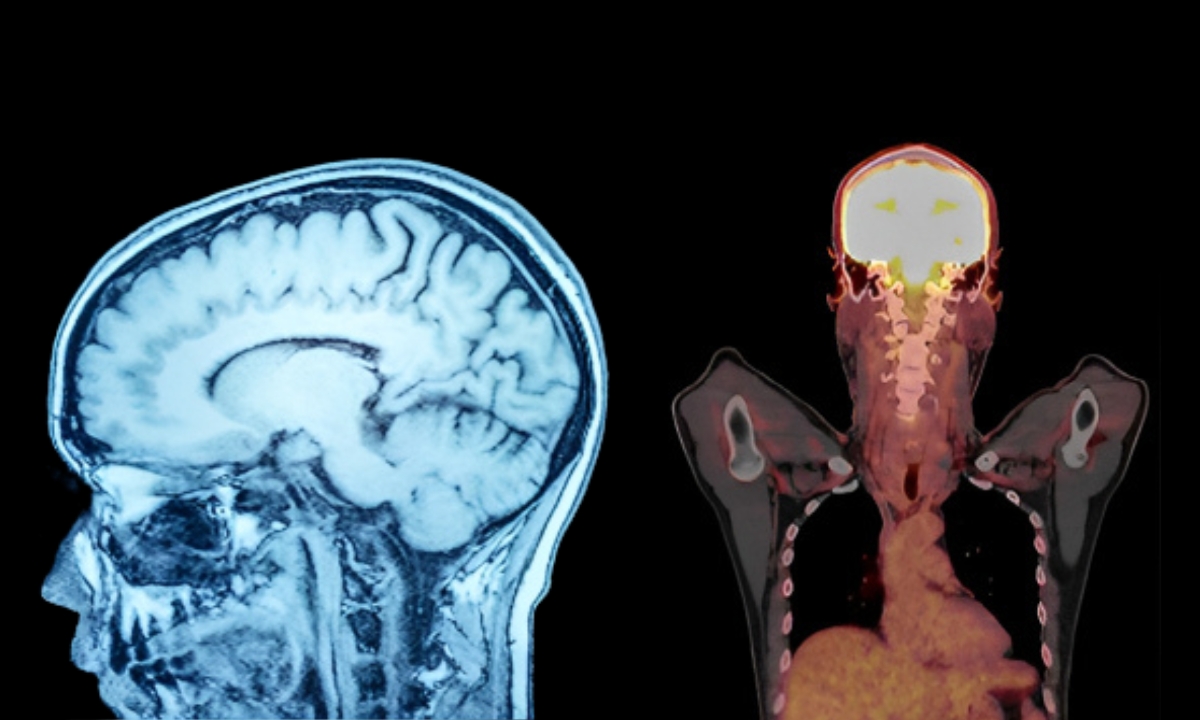
\includegraphics[width=0.6\textwidth]{ct-pet.png}
	\caption{A sinistra, un'immagine ottenuta tramite TAC; a destra, un'immagine ottenuta tramite PET.}
\end{figure}

\noindent Necessitando di visualizzare immagini sia anatomiche, che funzionali, si fa uso di appositi macchinari \textit{multimodali}, che permettono l'acquisizione contemporanea dei due tipi di immagini; ad esempio, esistono degli scan PET-CT.
Nell'acquisizione multimodale, una risonanza magnetica \`e tipicamente utilizzata per produrre un'immagine anatomica.

\subsection{Immagini digitali}


Un'immagine digitale \`e una matrice di numeri, che rappresentano l'intensit\`a del segnale misurato, oppure un valore derivato da modello. 
Complessivamente, le informazioni acquisite saranno composte da \textit{tre componenti} per immagini 2D (dimensione $x$, dimensione $y$, valore misurato) e da \textit{quattro componenti} per immagini 3D (dimensione $x$, dimensione $y$, dimensione $z$, valore misurato).
\`E anche possibile acquisire dati con 4 componenti, in cui al posto della terza dimensione, \`e inserito il tempo, in modo da ricreare l'evoluzione temporale di un'immagine bidimensionale.
Ogni matrice numerica costituisce un \textit{frame} dell'immagine.

\begin{boxenv}[]
	\centering Riprendere da pagina 16, -38:00\footnote{Fare prima da pagina 16 a 19, poi riprendere audio.}.
\end{boxenv}











\end{document}
